\documentclass{standalone}
\usepackage{graphicx}	
\usepackage{amssymb, amsmath}
\usepackage{color}

\usepackage{tikz}
\usetikzlibrary{intersections, backgrounds}
\usepackage{pgfmath}

\definecolor{light}{RGB}{220, 188, 188}
\definecolor{mid}{RGB}{185, 124, 124}
\definecolor{dark}{RGB}{143, 39, 39}
\definecolor{highlight}{RGB}{180, 31, 180}
\definecolor{gray10}{gray}{0.1}
\definecolor{gray20}{gray}{0.2}
\definecolor{gray30}{gray}{0.3}
\definecolor{gray40}{gray}{0.4}
\definecolor{gray60}{gray}{0.6}
\definecolor{gray70}{gray}{0.7}
\definecolor{gray80}{gray}{0.8}
\definecolor{gray90}{gray}{0.9}
\definecolor{gray95}{gray}{0.95}

\begin{document}

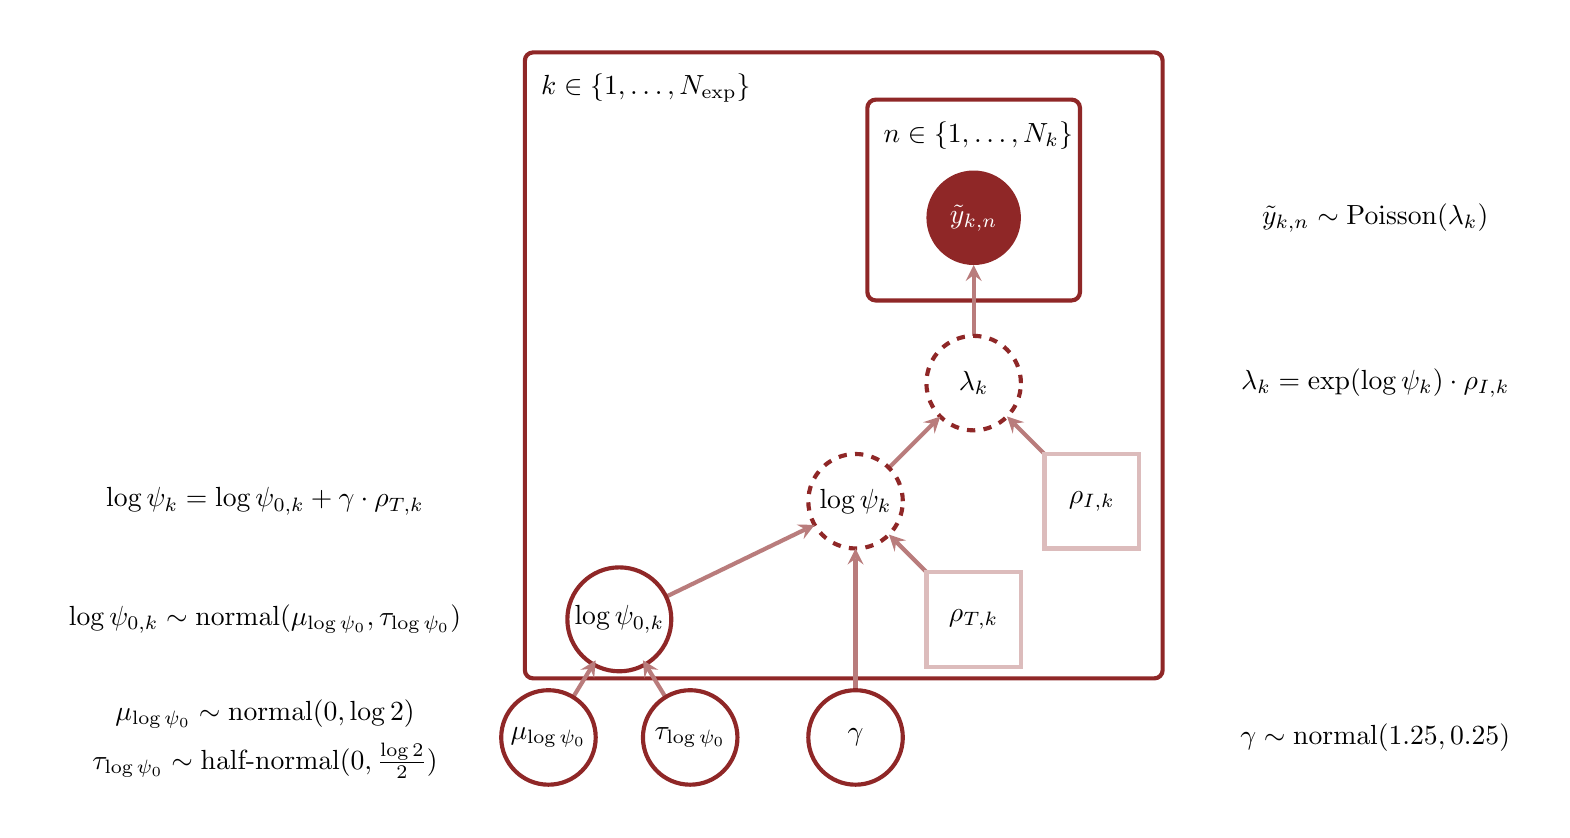
\begin{tikzpicture}[scale=0.3, thick]

\pgfmathsetmacro{\r}{2}

\draw[white] (-40, -18) rectangle (24, 15);

\filldraw[fill=white, draw=dark, line width=1.5, rounded corners=3pt] (-19, -12.5) rectangle (8, 14);

\node[right] at (-18.75, 12.5) { $k \in \{1, \ldots, N_{\mathrm{exp}} \}$ };

\filldraw[fill=white, draw=dark, line width=1.5, rounded corners=3pt] (-4.5, 3.5) rectangle (4.5, 12);

\node[right] at (-4.25, 10.5) { $n \in \{1, \ldots, N_{k} \}$ };

\fill[color=dark] (0, 7) circle (\r)
node[color=white] { $\tilde{y}_{k,n}$ };

\draw[->, >=stealth, color=mid, line width=1.5] (0, 0) -- (0, 7 - \r);

\filldraw[fill=white, draw=dark, dashed, line width=1.5] (0, 0) circle (\r)
node[color=black] { $\lambda_{k}$ };

\draw[->, >=stealth, color=mid, line width=1.5] (5, -5) -- ({0 + \r * cos(45)}, {0 - \r * sin(45)});

\filldraw[fill=white, draw=light, line width=1.5] (5 - \r, -5 - \r) rectangle +(2 * \r, 2 * \r);
\node at (5, -5) { $\rho_{I, k}$ };

\draw[->, >=stealth, color=mid, line width=1.5] (-5, -5) -- ({0 - \r * cos(45)}, {0 - \r * sin(45)});

\filldraw[fill=white, draw=dark, dashed, line width=1.5] (-5, -5) circle (\r)
node[color=black] { $\log \psi_{k}$ };

\draw[->, >=stealth, color=mid, line width=1.5] (0, -10) -- ({-5 + \r * cos(45)}, {-5 - \r * sin(45)});

\filldraw[fill=white, draw=light, line width=1.5] (0 - \r, -10 - \r) rectangle +(2 * \r, 2 * \r);
\node at (0, -10) { $\rho_{T, k}$ };

\draw[->, >=stealth, color=mid, line width=1.5] (-5, -15) -- (-5, -5 - \r);

\filldraw[fill=white, draw=dark, line width=1.5] (-5, -15) circle (\r)
node[color=black] { $\gamma$ };

\draw[->, >=stealth, color=mid, line width=1.5] (-15, -10) -- ({-5 - \r * cos(30)}, {-5 - \r * sin(30)});

\filldraw[fill=white, draw=dark, line width=1.5] (-15, -10) circle (1.1 * \r)
node[color=black] { $\log \psi_{0, k}$ };

\draw[->, >=stealth, color=mid, line width=1.5] (-18, -15) -- ({-15 - \r * cos(60)}, {-10 - \r * sin(60)});

\filldraw[fill=white, draw=dark, line width=1.5] (-18, -15) circle (\r)
node[color=black] { $\mu_{\log \psi_{0}}$ };

\draw[->, >=stealth, color=mid, line width=1.5] (-12, -15) -- ({-15 + \r * cos(60)}, {-10 - \r * sin(60)});

\filldraw[fill=white, draw=dark, line width=1.5] (-12, -15) circle (\r)
node[color=black] { $\tau_{\log \psi_{0}}$ };

\node[] at (17, 7)    { $\tilde{y}_{k,n} \sim \text{Poisson}(\lambda_{k})$ };
\node[] at (17, 0)    { $\lambda_{k} = \exp(\log \psi_{k}) \cdot \rho_{I, k}$ };
\node[] at (17, -15)    { $\gamma \sim \text{normal}(1.25, 0.25)$ };

\node[] at (-30, -5)  { $\log \psi_{k} = \log \psi_{0, k} + \gamma \cdot \rho_{T, k}$ };
\node[] at (-30, -10)  { $\log \psi_{0, k} \sim \text{normal}(\mu_{\log \psi_{0}}, \tau_{\log \psi_{0}})$ };
\node[] at (-30, -14)  { $\mu_{\log \psi_{0}} \sim \text{normal}(0, \log 2)$ };
\node[] at (-30, -16)  { $\tau_{\log \psi_{0}} \sim \text{half-normal}(0, \frac{\log 2}{2} )$ };

\end{tikzpicture}

\end{document}  